\documentclass[a4paper,10pt, twocolumn]{article}
\usepackage{amsmath}
\usepackage{graphicx}
\usepackage[font={small,it}]{caption}



\begin{document}

\title{Linear Regression on Boston Housing Data}
\author{Alun Meredith}
\maketitle

\section{Method}
In both linear regression and Radial Basis Functions (RBF) we construct a model of the data and train that model to best represent the data; minimising an error function representing the distance between the observations the model. Linear regression models distributions around a straight line model whereas LBF models distributions ($\phi$)  around a collection of points (eq.\ref{eq:model}).

\begin{align}
	\label{eq:model}	
	g(\mathbf{x}) &= \sum_{k=1}^K\lambda_k\phi(||\mathbf{x-c_k}||)\\
	\label{eq:pdf}
	\phi(c_k,x) &= e^{{-\frac{(x-c_k)^2}{2\sigma^2}}}\\
	\label{eq:weights}
	\lambda &= D / y
\end{align} 

To construct a regression using RBF we first normalise the data. The purpose of normalising the data is the make sure that variables with large values don't dominate variables with small values. 

Evaluating the position of the centres a K-means clustering algorithm was used. This algorithm doesn't always converge to a global optimum. As such it can be worth repeating reinitialising the algorithm to find better solutions.

The distribution away from the model must be chosen. These distributions are the 'Radial Basis Functions'; different functions can be chosen to model the data in different ways. In this case we chose a Gaussian model (eq.\ref{eq:pdf}) which confers a sense of locality. We estimate $\sigma$ as the average of a sample of 10 distances between random observations.

Using these RBFs compute the probability density of each of the K centres on each of the n observations (eq.\ref{eq:pdf}) to construct a design matrix $D$. Train the weights ($\lambda$) of each Radial basis function as the effect its PDF has on the target value $y$ (eq.\ref{eq:weights}).
\section{Parameters}

This model has two parameters, the number of clusters $K$ and the variance of the Gaussian RBF $\sigma$. To evaluate these values in hierarchical clustering a dendrogram can be used and low dimensional data can be visually inspected. Here however we cannot use those techniques so we vary the values of both of these parameters and choose the value with greatest performance on the test set.

\begin{figure}[t]
	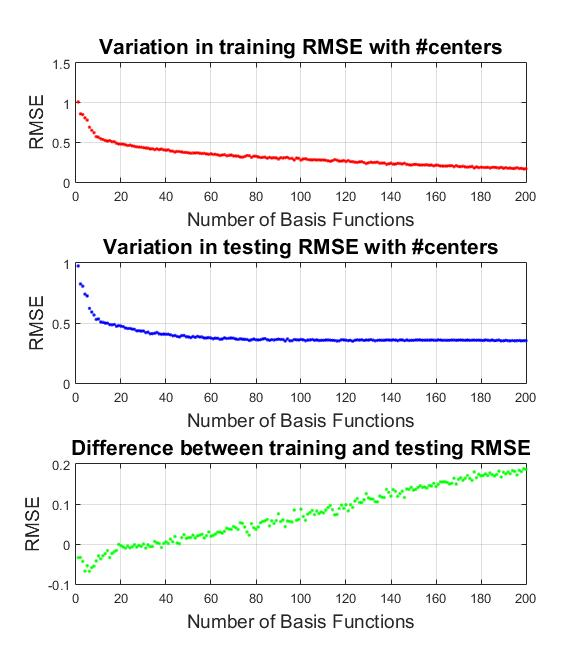
\includegraphics[width=0.7\linewidth]{VaryingK.jpg}
	\centering
	\caption{Variation in testing and training RMSE error with number of RBF clusters K}
		\label{fig:VaryingK}
\end{figure}

By varying the number of clusters figure (\ref{fig:VaryingK}) shows that the training set continuously improves accuracy as the model becomes more complex but this no longer has an effect on unseen data. This indicates high variance, with high bias present when the model is too simple and performs poorly on both set. We choose the smallest number of centres which where the testing set RMSE no longer improves substantially in this case around 50. 

\begin{figure}[ht]
	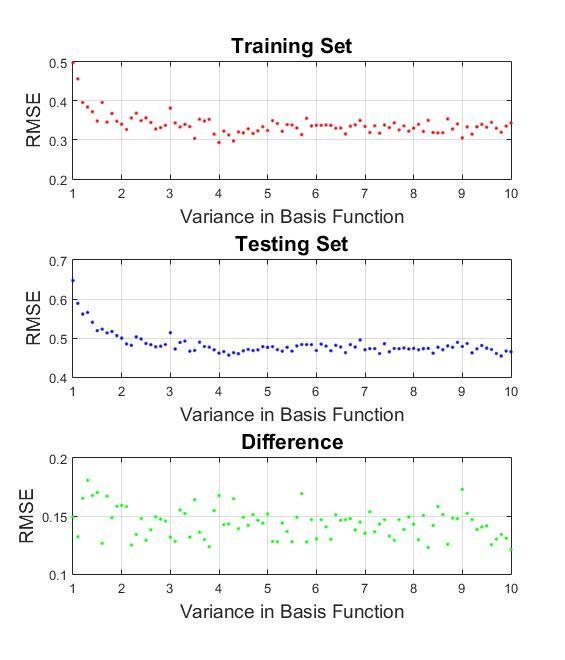
\includegraphics[width=0.7\linewidth]{VaryingSigma.jpg}
	\centering
	\caption{Variation in testing and training RMSE error with variance of Basis Functions $\sigma$}
		\label{fig:varyingSigma}
\end{figure}

Varying the value of sigma (fig. \ref{fig:varyingSigma}) similarly shows poor performance at low values however at high values neither set sees any noticeable change after a value in the range of 3-5. Considering the average value approximated earlier fell in this range (4.70) we will continue to use it.

\section{Contrast with Linear Model}

When comparing our RBF to the linear model Figure \ref{fig:linearComparison} shows the linear regression outperforming the non-linear RBF regression on the training set but significantly under-performing on the validation set. This demonstrates that linear regression is much more susceptible to variance than the RBF however if you average the validation set models for linear regression you get a RMSE on a test set of 0.14, outperforming the radial basis function. We cannot use a similar method for the RBF because the K-means algorithm isn't deterministic. 

\begin{figure}[ht]
	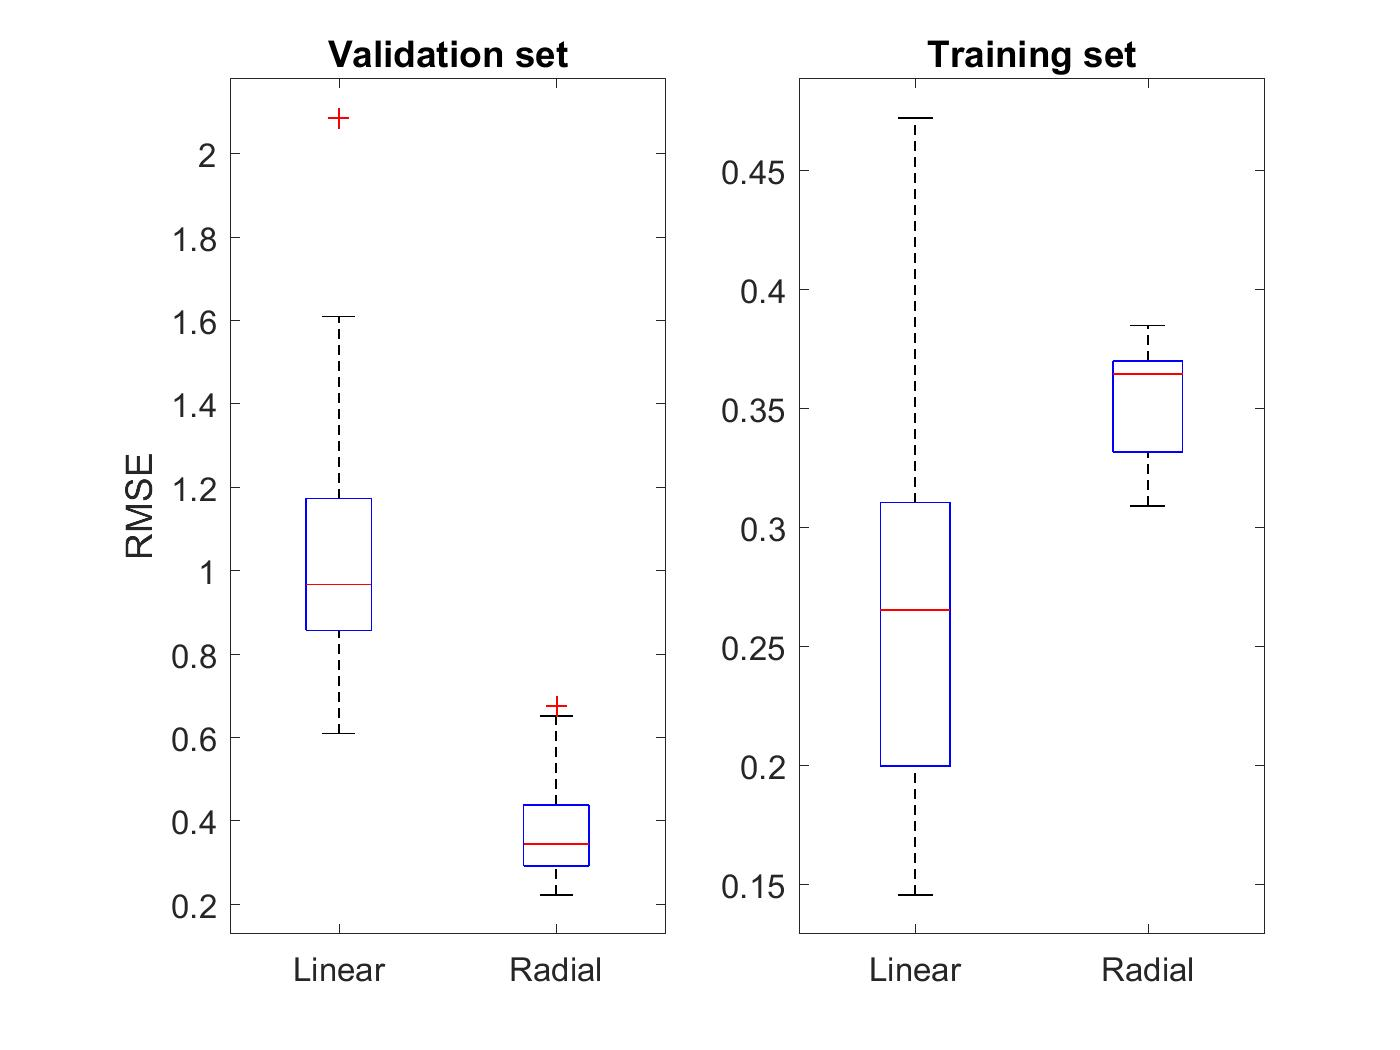
\includegraphics[width=0.7\linewidth]{linearComparison.jpg}
	\centering
	\caption{Comparison between linear and RBF models on house prices for RMSE from 10 fold cross-validation}
		\label{fig:linearComparison}
\end{figure}

\section{Wine Dataset\cite{wineQuality}}

Finally we have repeated these steps to produce models of the quality of red wine. Repeating the methods used for the Boston housing data we get similar results (not shown for space reasons). 

\begin{figure}[ht]
	\includegraphics[width=0.7\linewidth]{wineResults.jpg}
	\centering
	\caption{Prediction accuracy of RBF on one of the validation folds for Wine Quality data}
		\label{fig:WineResults}
\end{figure}

It can be seen from figure \ref{fig:WineResults} above that the wine dataset is much less accurate using RBF than previously, at least some of this can be attributed to the categorical nature of the results. It would make more sense to round our predictions to the nearest category for example or change the RBF to reflect the distribution of the data. 

\begin{table}[b]
\begin{tabular}{l c|c|c|c}
	
	&  & Test & validation & train \\
Housing	& Linear & 1.14 & 1.07 & 0.27 \\
	& RBF & 0.38 & & 0.35 \\
Wine& Linear & 0.42 & 0.90 & 0.73 \\
	& RBF & 0.79 & & 0.77 \\
\end{tabular}
\caption{RMSE errors for both Boston Housing Data and Wine Quality data using linear and RBF models with 50 centres and 20 fold cross-validation}
\end{table}
 
\begin{thebibliography}{9}
\bibitem{wineQuality}
  Leslie Lamport et al.,
  Modeling wine preferences by data mining, %from physicochemical properties, 
  %In Decision Support Systems, 
  %Elsevier, 
  %47(4):547-553, 
  2009.
\end{thebibliography}
\end{document}